\documentclass[11pt,letterpaper,oneside]{article}
\usepackage[top=0.5in,left=1in,right=1in,bottom=1in]{geometry}
%\usepackage[top=0.5in,left=1.8in,right=1.8in,bottom=1in]{geometry}
\usepackage{fancyvrb}
\usepackage{colortbl}
\usepackage[pdftex]{graphicx}
\DeclareGraphicsExtensions{.pdf}
\usepackage{url}
\usepackage{amsmath}

%\usepackage{setspace}
%\doublespacing

\title{Homework 3}
\author{Dejun Qian}

\date{}

\begin{document}
\maketitle

\begin{description}

\item[Experiment 1:] The accuracy of the trained SVM is 89.62\% (3299 correct, 382 incorrect, 3681 total). The ROC curve is shown in Figure~\ref{fig1}.

From the ROC curve, we can see that the SVM is not stronger on either positive examples or negative examples.

\begin{figure}
\begin{center}
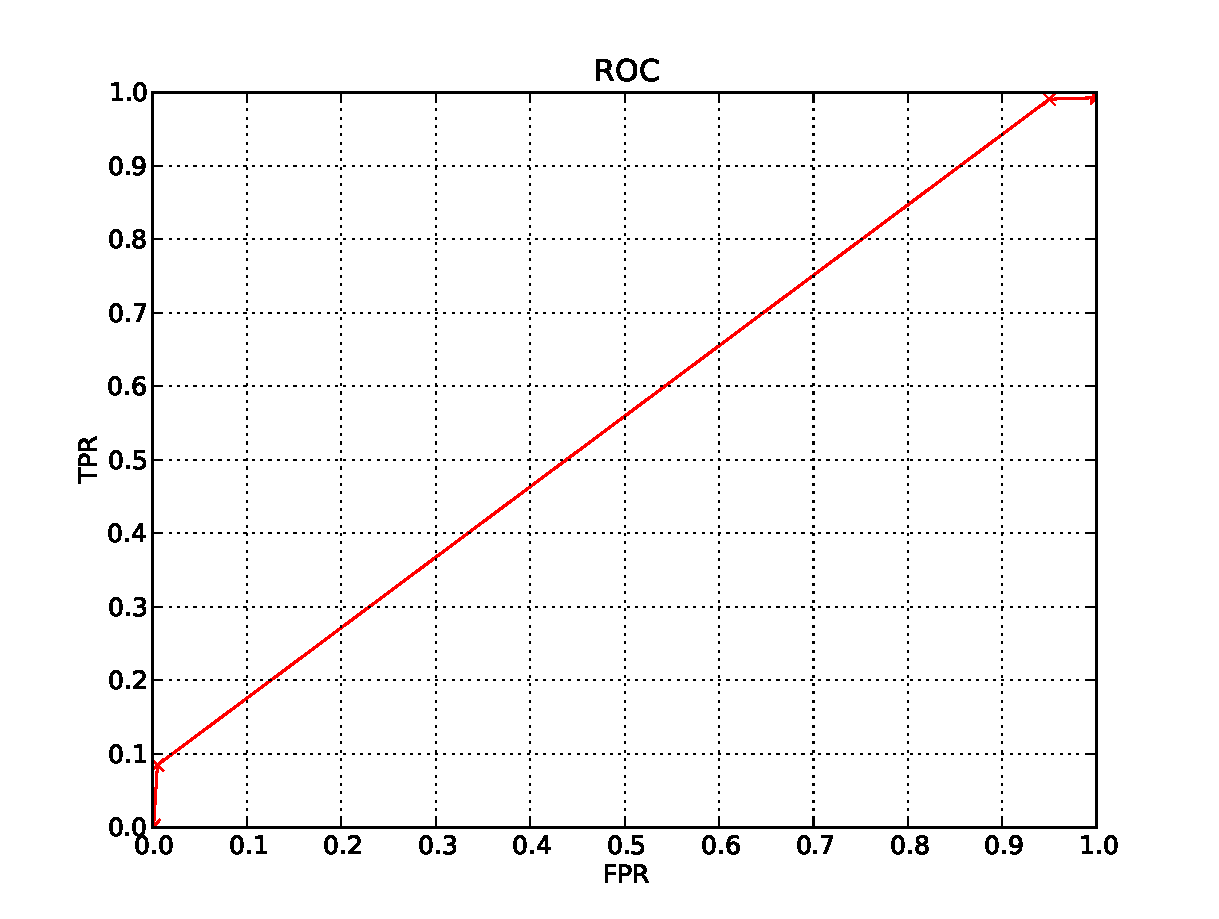
\includegraphics[width=0.55\textwidth]{fig1}
\caption{Experiment 1}
\label{fig1}
\end{center}
\end{figure}

\item[Experiment 2:] The accuracy of the ensemble SVM when $K=10$ is 87.31\% (3214 correct, 467 incorrect, 3681 total). The accuracy is less than the result in experiment 1, which means ensemble classifier does not always better. The ROC curve is shown in Figure~\ref{fig2}.

From the ROC curve, we can see that the ensemble SVM is not stronger on either positive examples or negative examples.

The ROC curve is different from the result from experiment 1. The values of TPR and FPR are more continuous.

\begin{figure}
\begin{center}
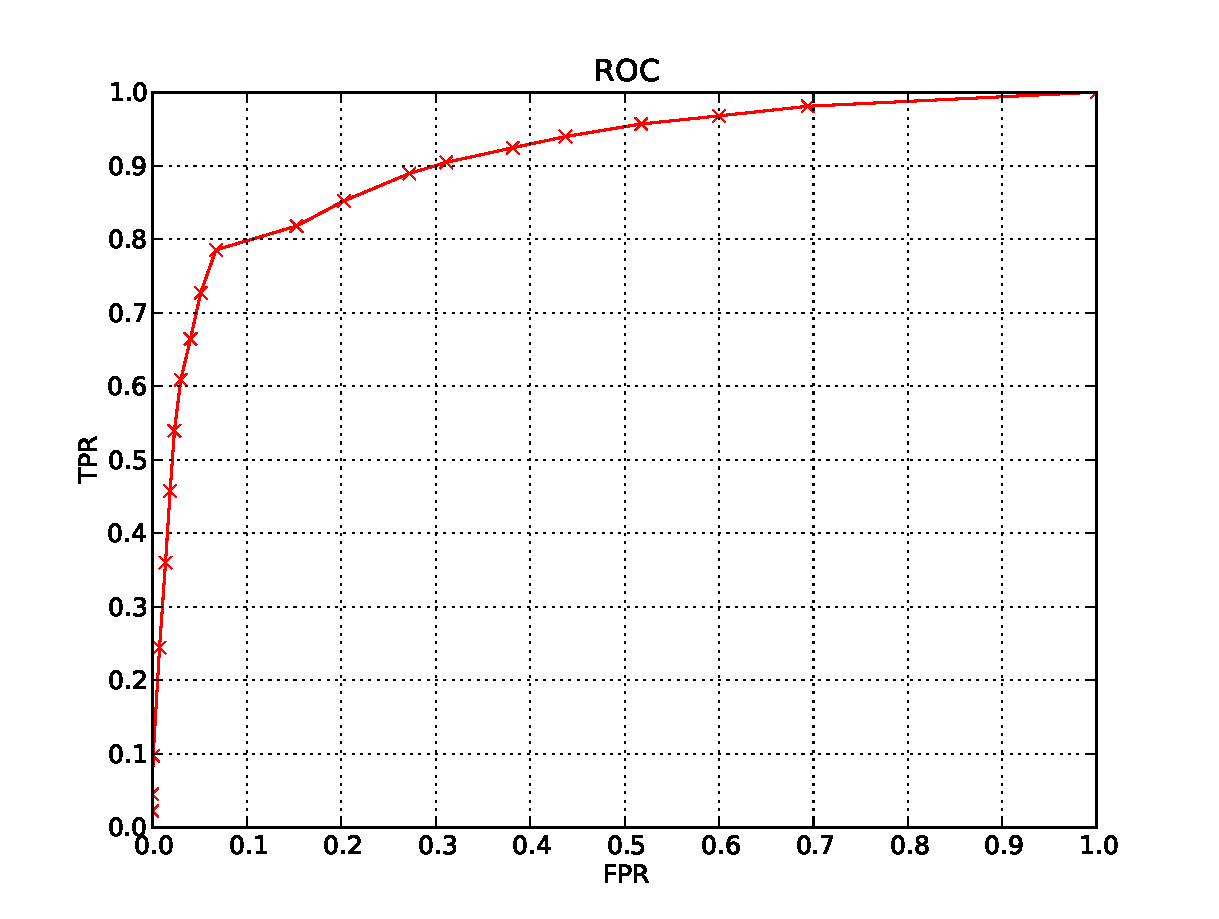
\includegraphics[width=0.55\textwidth]{fig2}
\caption{Experiment 2}
\label{fig2}
\end{center}
\end{figure}

\item[Experiment 3:] The accuracy on the ensemble SVM when $K=20$ is 88.32\% (3251 correct, 430 incorrect, 3681 total). The accuracy is a little bit better than experiment 2, and still less than experiment 1. The ROC curve is shown in Figure~\ref{fig3}.

From the ROC curve, we can see that the ensemble SVM is not stronger on either positive examples or negative examples.

The ROC curve is also different from the result from experiment 1. The values of TPR and FPR are more continuous. Compared to experiment 2, the ROC is a litter bit better.

\begin{figure}
\begin{center}
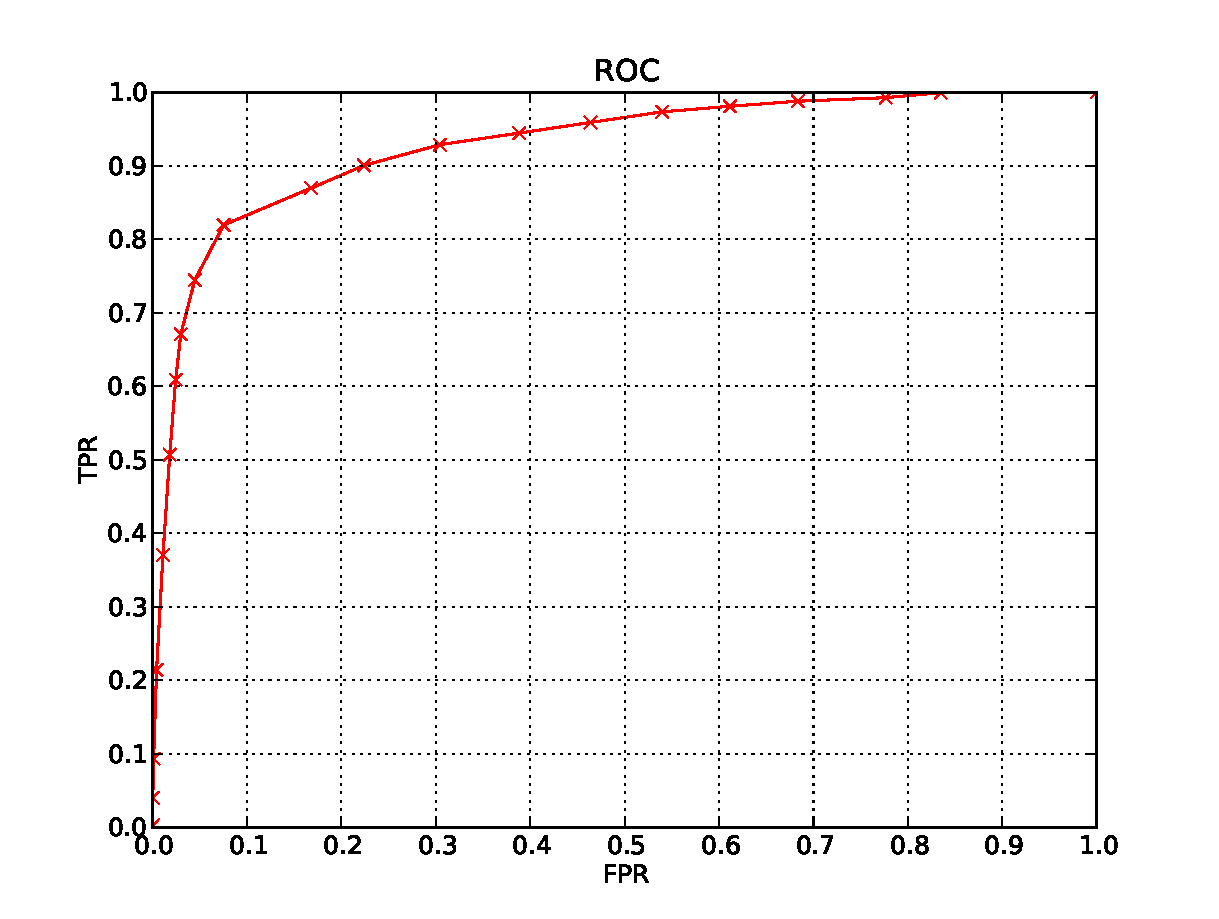
\includegraphics[width=0.55\textwidth]{fig3}
\caption{Experiment 3}
\label{fig3}
\end{center}
\end{figure}

\end{description}

In conclusion, the result of ensemble SVM is not always better than the single SVM. More iterations do help improve the accuracy and ROC curve.

\end{document}
